%% \section{Discussion}\label{sec:discussion}
%% \stitle{Faithfullness}
%% A natural question is to ask why gradients of counterfactuals obtained
%% by scaling the input capture feature importance for the original image.
%% First, from
%% studying the visualizations in Figure~\ref{fig:intgrad-finalgrad},
%% the results look reasonable in that the highlighted pixels capture features
%% representative of the predicted class as a human would perceive
%% them. Second, we confirmed that the network too seems to find these
%% features representative by performing ablations.
%% %Specifically, we
%% %ablate the smallest bounding box drawn around the pixels that are in
%% %the top $5\%$ by importance score, and observe that the softmax score for
%% %the class drops significantly.
%% It is somewhat natural to expect that the Inception network is robust to
%% to changes in input intensity; presumably there are some low brightness images
%% in the training set.

%% However, these counterfactuals seem reasonable even for
%% networks where such scaling does not correspond to a natural concept
%% like intensity, and when the counterfactuals fall outside the training
%% set; for instance in the case of the ligand-based virtual screening network (see
%% Section~\ref{sec:drug-discovery}).
%% We \emph{speculate} that the reason why these counterfactuals
%% make sense is because the network is built by composing ReLUs.
%% As one scales the input starting from a suitable baseline, various
%% neurons activate, and the scaling process that does a somewhat thorough
%% job of exploring all these events that contribute to the prediction for the
%% input. There is an analogous argument for other operator such as max pool,
%% average pool, and softmax---here the triggering events aren’t discrete
%% but the argument is analogous.

%% %% \stitle{Generation vs. Discrimination}
%% %% In generative models, all features contribute to single task. In this
%% %% respect, gradients effectively quantify the importance of each feature
%% %% to the final prediction score.

%% %% On the other hand in discriminative models (such ones with a softmax
%% %% classifier output), features contribute to multiple tasks which are
%% %% all competing against each other. A feature may be important for task
%% %% in two ways, either directly by contributing to the prediction for the
%% %% task, or indirectly by hurting the prediction of other tasks. Features
%% %% importance quantified by gradients does not distinguish between such
%% %% direct and indirect contributions, which makes it challenging to
%% %% interpret.

%% \stitle{Limitations of Approach}
%% We discuss some limitations of our technique; in a sense these are
%% limitations of the problem statement and apply equally to other
%% techniques that attribute to base input features.
%% \begin{itemize}
%% \item \textbf{Inability to capture Feature interactions:} The models could
%%   perform logic that effectively combines features via a conjunction or
%%   an implication-like operations; for instance, it could be that a
%%   molecule binds to a site if it has a certain structure that is
%%   essentially a conjunction of certain atoms and certain bonds
%%   between them. Attributions or importance scores have no way to
%%   represent these interactions.
%% \item \textbf {Feature correlations:} Feature correlations are a bane to the
%%   understandability of all machine learning models. If there are two
%%   features that frequently co-occur, the model is free to assign
%%   weight to either or both features. The attributions would then respect
%%   this weight assignment. But, it could be that the specific weight
%%   assignment chosen by the model is not human-intelligible. Though
%%   there have been approaches to feature selection that reduce feature
%%   correlations (\cite{YL03}), it is unclear how they apply to deep models
%%   on dense input.
%% \end{itemize}

%% \stitle{When Interior Gradients and Gradients at the image coincide}
%% If the network only consists of RELUs with zero biases, Max/Avg pool nodes,
%% then the function is linear in the scaling of intensities, i.e., all
%% the interior gradients are identical. (Notice that this does not imply
%% that the network is a linear function of its input, just that it is
%% linear to such uniform scaling of intensities.) So it is tempting to
%% quantify feature importance using just the gradient of the input for
%% such networks. But this comes with a caveat. It could still be that
%% the network contrives biases by hiding them in input features. This is
%% easier to see if the network relies on an embedding representation of
%% the input. It could simply use an embedding dimension as a constant
%% and propagate this constant to higher level layers. This would distort
%% the gradient in a way that makes it not reflective of feature
%% importance. Notice this phenomenon could also occur in networks with
%% RELUs that have non zero biases. Although, one would hope that it
%% isn’t as frequent in such networks as the bias variable are available.

\section{Other Related work}\label{sec:related}
We already covered closely related work on attribution in
Section~\ref{sec:two-axioms}.  We mention other related work.
Over the last few years, there has been a vast amount work on
demystifying the inner workings of deep networks. Most of this work
has been on networks trained on computer vision tasks, and deals with
understanding what a specific neuron computes~\cite{EBCV09, QVL13}
and interpreting the representations captured by neurons during a
prediction~\cite{MV15, DB15, YCNFL15}. In contrast, we focus on
understanding the network's behavior on a specific input in terms of
the base level input features. Our technique quantifies the importance
of each feature in the prediction.


 One approach to the attribution problem proposed first
 by~\cite{RSG16a, RSG16b}, is to locally approximate the behavior of
 the network in the vicinity of the input being explained with a
 simpler, more interpretable model.  An appealing aspect of this
 approach is that it is completely agnostic to the implementation of
 the network and satisfies implemenation invariance. However, this
 approach does not guarantee sensitivity. There is no guarantee that
 the local region explored escapes the ``flat'' section of the
 prediction function in the sense of Section~\ref{sec:two-axioms}. The other
 issue is that the method is expensive to implement for networks with
 ``dense'' input like image networks as one needs to explore a local
 region of size proportional to the number of pixels and train a model
 for this space. In contrast, our technique works with a few calls to
 the gradient operation.

Attention mechanisms~\cite{BahdanauCB14} have gained popularity recently. One may think that
attention could be used a proxy for attributions, but this has issues. For instance, in a LSTM that also employs attention, there are many ways for an input token to influence an output token: the memory cell, the recurrent state, and ``attention''.
Focussing only an attention ignores the other modes of influence and results in an incomplete picture. 

 
%% \begin{figure}[!htb]
%%   \centering
%%   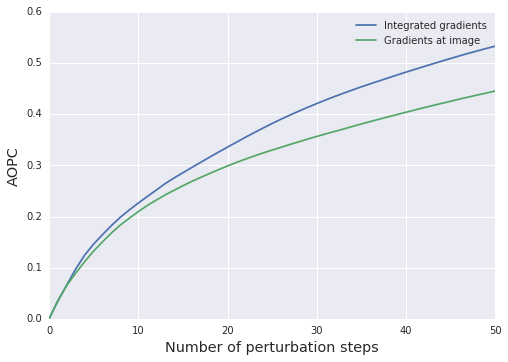
\includegraphics[width=0.5\columnwidth]{Figures/AOPC/aopc.png}
%%   \caption{AOPC (\cite{SBMBM15}) for integrated gradients and gradients at image.}\label{fig:aopc}
%% \end{figure}

%% \begin{figure}
%%   \centering
%%   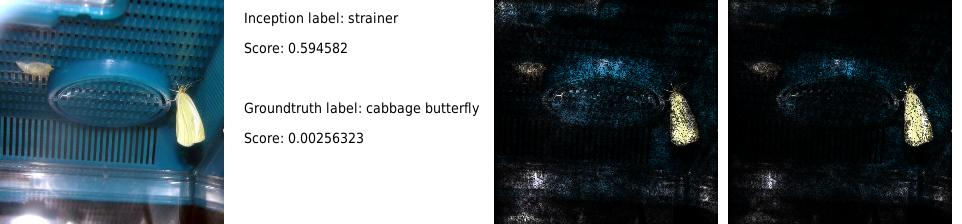
\includegraphics[width=0.7\columnwidth]{Figures/Misclassified/cabbage_butterfly.jpg}
%%   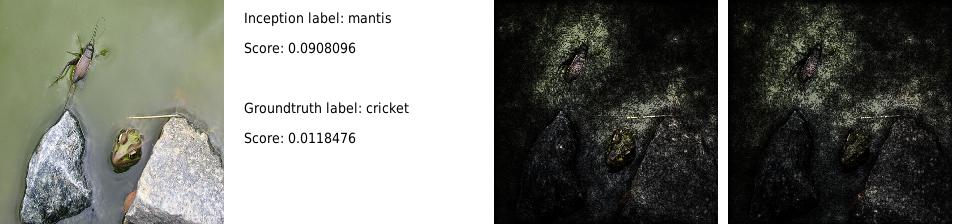
\includegraphics[width=0.7\columnwidth]{Figures/Misclassified/mantis.jpg}
%%   \caption{\textbf{Interior gradients of misclassified images.} Left-to-right: Original image,
%%     Softmax score for the top label assigned by the Inception network and the groundtruth
%%     label provided by ImageNet, visualization of integrated gradients w.r.t. Inception label,
%%     visualization of integrated gradients w.r.t. groundtruth label.}\label{fig:attribution-mis}
%% \end{figure}
